\fbox{\begin{minipage}[t]{1\textwidth}
    \scriptsize
    \textbf{Binary Search Trees (BST)}\\[2pt]
    \textbf{Properties:}
    \begin{minipage}[t]{0.65\textwidth}
        \begin{itemize}
        \item[-] Left subtree: all keys < node's key
        \item[-] Right subtree: all keys > node's key
        \item[-] Left and right subtrees are also BSTs
        \item[-] A \textbf{Node} has: \textbf{key} (value), \textbf{left} \& \textbf{right} (child pointers), \textbf{parent} (optional)
        \end{itemize}
    \end{minipage}
    \vspace{2pt}
    
    \begin{minipage}[t]{0.19\textwidth}
        \centering
        \textbf{\scriptsize BST-Search}\\[2pt]
        \scriptsize
        \begin{minipage}[t]{\textwidth}
            \scriptsize
            1. Start at root\\
            2. If NULL, return NULL\\
            3. If key = root's key, return root\\
            4. If key < root's key, search left\\
            5. If key > root's key, search right
        \end{minipage}\\[3pt]
        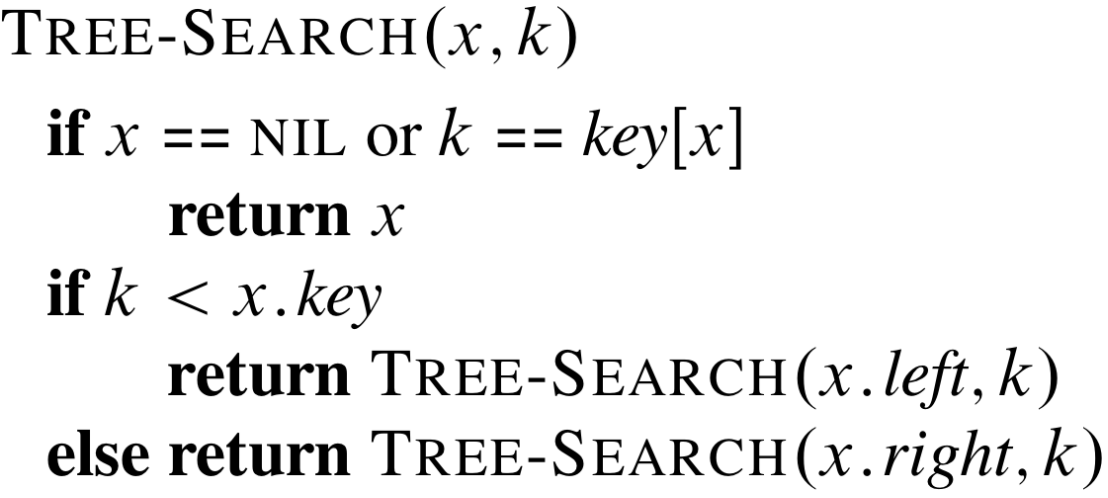
\includegraphics[width=0.85\textwidth]{images/bst-search.png}\\[2pt]
        \textit{Time:} \(O(\log n)\) avg, \(O(n)\) worst\\
        \textit{Space:} \(O(\log n)\)
    \end{minipage}
    \hfill
    \begin{minipage}[t]{0.19\textwidth}
        \centering
        \textbf{\scriptsize BST-Minimum}\\[2pt]
        \scriptsize
        \begin{minipage}[t]{\textwidth}
            \scriptsize
            1. Start at root\\
            2. If NULL, return NULL\\
            3. Follow left pointers until no left child\\
            4. Return leftmost node
        \end{minipage}\\[8pt]
        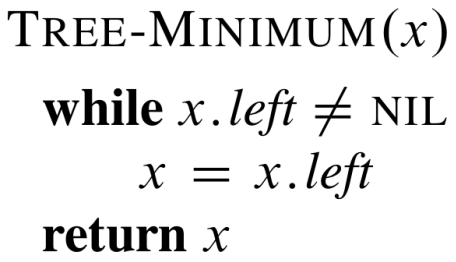
\includegraphics[width=0.5\textwidth]{images/bst-minimum.png}\\[2pt]
        \textit{Time:} \(O(h)\)\\
        \textit{Space:} \(O(1)\)
    \end{minipage}
    \hfill
    \begin{minipage}[t]{0.19\textwidth}
        \centering
        \textbf{\scriptsize BST-Maximum}\\[2pt]
        \scriptsize
        \begin{minipage}[t]{\textwidth}
            \scriptsize
            1. Start at root\\
            2. If NULL, return NULL\\
            3. Follow right pointers until no right child\\
            4. Return rightmost node
        \end{minipage}\\[8pt]
        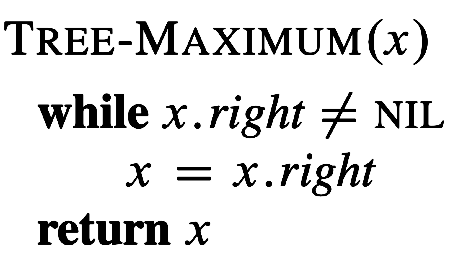
\includegraphics[width=0.5\textwidth]{images/bst-maximum.png}\\[2pt]
        \textit{Time:} \(O(h)\)\\
        \textit{Space:} \(O(1)\)
    \end{minipage}
    \hfill
    \begin{minipage}[t]{0.19\textwidth}
        \centering
        \textbf{\scriptsize BST-Successor}\\[2pt]
        \scriptsize
        \begin{minipage}[t]{\textwidth}
            \scriptsize
            1. If right subtree exists:\\
            \quad Return minimum in right subtree\\
            2. Otherwise:\\
            \quad Find first ancestor where\\
            \quad node is in left subtree
        \end{minipage}\\[4pt]
        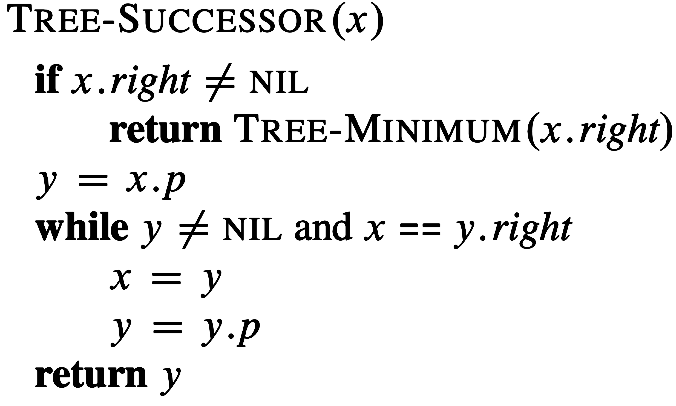
\includegraphics[width=0.8\textwidth]{images/bst-successor.png}\\[2pt]
        \textit{Time:} \(O(h)\)\\
        \textit{Space:} \(O(1)\)
    \end{minipage}
    \hfill
    \begin{minipage}[t]{0.19\textwidth}
        \centering
        \textbf{\scriptsize BST-Predecessor}\\[2pt]
        \scriptsize
        \begin{minipage}[t]{\textwidth}
            \scriptsize
            1. If left subtree exists:\\
            \quad Return maximum in left subtree\\
            2. Otherwise:\\
            \quad Find first ancestor where\\
            \quad node is in right subtree
        \end{minipage}\\[4pt]
        \textit{Time:} \(O(h)\)\\
        \textit{Space:} \(O(1)\)
    \end{minipage}
\end{minipage}} 